\documentclass{beamer}
\usepackage[utf8]{inputenc}
\usepackage{graphicx, epsfig}
\usepackage{amsmath,mathrsfs,amsfonts,amssymb}
\usepackage{floatflt}
\usepackage{epic,ecltree}
\usepackage{mathtext}
\usepackage{fancybox}
\usepackage{fancyhdr}
\usepackage{multirow}
\usepackage{enumerate}
\usepackage{epstopdf}
\usepackage{multicol}
\usepackage{algorithm}
\usepackage[noend]{algorithmic}
\usepackage{tikz}
\usepackage{blindtext}
\usetheme{default}%{Singapore}%{Warsaw}%{Warsaw}%{Darmstadt}
\usecolortheme{default}

\setbeamerfont{title}{size=\Huge}
\setbeamertemplate{footline}[page number]{}

\setbeamertemplate{section in toc}[sections numbered]


\makeatletter
\newcommand\HUGE{\@setfontsize\Huge{35}{40}}
\makeatother    

\setbeamerfont{title}{size=\HUGE}
\beamertemplatenavigationsymbolsempty

% latin bold lower
\newcommand{\ba}{\mathbf{a}} 
\newcommand{\bc}{\mathbf{c}} 
\newcommand{\be}{\mathbf{e}} 
\newcommand{\bh}{\mathbf{h}} 
\newcommand{\bp}{\mathbf{p}} 
\newcommand{\bt}{\mathbf{t}} 
\newcommand{\bs}{\mathbf{s}} 
\newcommand{\bu}{\mathbf{u}} 
\newcommand{\bv}{\mathbf{v}} 
\newcommand{\bw}{\mathbf{w}} 
\newcommand{\bx}{\mathbf{x}} 
\newcommand{\by}{\mathbf{y}} 
\newcommand{\bz}{\mathbf{z}} 

% latin bold upper
\newcommand{\bA}{\mathbf{A}} 
\newcommand{\bB}{\mathbf{B}} 
\newcommand{\bC}{\mathbf{C}} 
\newcommand{\bI}{\mathbf{I}} 
\newcommand{\bJ}{\mathbf{J}} 
\newcommand{\bL}{\mathbf{L}} 
\newcommand{\bM}{\mathbf{M}} 
\newcommand{\bP}{\mathbf{P}}
\newcommand{\bQ}{\mathbf{Q}} 
\newcommand{\bR}{\mathbf{R}} 
\newcommand{\bT}{\mathbf{T}} 
\newcommand{\bU}{\mathbf{U}} 
\newcommand{\bV}{\mathbf{V}} 
\newcommand{\bW}{\mathbf{W}} 
\newcommand{\bX}{\mathbf{X}} 
\newcommand{\bY}{\mathbf{Y}} 
\newcommand{\bZ}{\mathbf{Z}} 

% latin cal upper
\newcommand{\cF}{\mathcal{F}} 
\newcommand{\cG}{\mathcal{G}} 
\newcommand{\cI}{\mathcal{I}} 
\newcommand{\cL}{\mathcal{L}} 
\newcommand{\cM}{\mathcal{M}} 
\newcommand{\cN}{\mathcal{N}} 
\newcommand{\cS}{\mathcal{S}} 
\newcommand{\cT}{\mathcal{T}} 
\newcommand{\cW}{\mathcal{W}} 
\newcommand{\cX}{\mathcal{X}} 
\newcommand{\cZ}{\mathcal{Z}} 

% latin bb upper
\newcommand{\bbE}{\mathbb{E}} 
\newcommand{\bbI}{\mathbb{I}} 
\newcommand{\bbP}{\mathbb{P}} 
\newcommand{\bbR}{\mathbb{R}} 

% greek bold lower
\newcommand{\bepsilon}{\boldsymbol{\epsilon}} 
\newcommand{\btheta}{\boldsymbol{\theta}} 
\newcommand{\blambda}{\boldsymbol{\lambda}} 
\newcommand{\bpi}{\boldsymbol{\pi}} 
\newcommand{\bmu}{\boldsymbol{\mu}} 
\newcommand{\bsigma}{\boldsymbol{\sigma}} 
\newcommand{\bphi}{\boldsymbol{\phi}} 

% greek bold upper
\newcommand{\bSigma}{\boldsymbol{\Sigma}} 

\DeclareMathOperator*{\argmin}{arg\,min}
\DeclareMathOperator*{\argmax}{arg\,max}

\newcommand{\createdgmtitle}[1]{\title[\hbox to 56mm{Deep Generative Models  \hfill\insertframenumber\,/\,\inserttotalframenumber}]
	{Deep Generative Models \\ {\Huge Lecture #1}}
	\author{Roman Isachenko}
	\institute{
\includegraphics[width=0.5cm]{../utils/ozonmasterslogo} \large{Ozon Masters}}
	\date{Spring, 2022}
}

\usepackage{tikz}
\usetikzlibrary{arrows,shapes,positioning,shadows,trees}

\newcommand\myfootnote[1]{%
  \tikz[remember picture,overlay]
  \draw (current page.south west) +(1in + \oddsidemargin,0.5em)
  node[anchor=south west,inner sep=0pt]{\parbox{\textwidth}{%
      \rlap{\rule{10em}{0.4pt}}\raggedright\scriptsize \textit{#1}}};}

\newcommand\myfootnotewithlink[2]{%
  \tikz[remember picture,overlay]
  \draw (current page.south west) +(1in + \oddsidemargin,0.5em)
  node[anchor=south west,inner sep=0pt]{\parbox{\textwidth}{%
      \rlap{\rule{10em}{0.4pt}}\raggedright\scriptsize\href{#1}{\textit{#2}}}};}
      
\AtBeginSection[]
{
	\begin{frame}{Outline}
		\tableofcontents[currentsection,subsectionstyle=hide]
	\end{frame}
}
\AtBeginSubsection[]{
	\begin{frame}{Outline}
		\tableofcontents[currentsection,currentsubsection]
	\end{frame}
}
\createdgmtitle{8}
\usepackage{tikz}

\usetikzlibrary{arrows,shapes,positioning,shadows,trees}
%--------------------------------------------------------------------------------
\begin{document}
%--------------------------------------------------------------------------------
\begin{frame}[noframenumbering,plain]
%\thispagestyle{empty}
\titlepage
\end{frame}
%=======
\begin{frame}{Recap of previous lecture}
	Let our data $\by$ comes from discrete distribution $\Pi(\by)$.
	\begin{block}{Discrete model}
		\begin{itemize}
			\item Use \textbf{discrete} model (e.x. $P(\by | \btheta) = \text{Cat}(\bpi(\btheta))$). 
			\item Minimize any suitable divergence measure $D(\Pi, P)$.
		\end{itemize}
	\end{block}
	\vspace{-0.2cm}
	\begin{block}{Continuous model}
		Use \textbf{continuous} model (e.x. $p(\bx | \btheta) = \cN(\bmu_{\btheta}(\bx), \bsigma_{\btheta}^2(\bx))$), but
			\begin{itemize}
				\item \textbf{discretize} model (make the model outputs discrete): transform $p(\bx | \btheta)$ to $P(\by | \btheta)$;
				\item \textbf{dequantize} data (make the data continuous): transform $\Pi(\by)$ to $\pi(\bx)$.
			\end{itemize}
	\end{block}
	\vspace{-0.2cm}
	\begin{block}{Model discretization through CDF}
		\vspace{-0.5cm}
		\[
			F(\bx | \btheta) = \int_{-\infty}^{\bx} p(\bx' | \btheta) d\bx'; \quad 
			P(\by | \btheta) = F(\by + 0.5 | \btheta) - F(\by - 0.5 | \btheta)
		\]
	\end{block}
	
	\myfootnotewithlink{https://arxiv.org/abs/1701.05517}{Salimans T. et al. PixelCNN++: Improving the PixelCNN with Discretized Logistic Mixture Likelihood and Other Modifications, 2017}\end{frame}
%=======
\begin{frame}{Recap of previous lecture}
	\begin{block}{Uniform dequantization bound}
		Let dequantize discrete distribution $\Pi(\by)$ to continuous distribution $\pi(\bx)$ in the following way: $\bx = \by + \bu$, where  $\bu \sim U[0, 1]$.
	\end{block}
	\begin{block}{Theorem}
	Fitting continuous model $p(\bx | \btheta)$ on uniformly dequantized data is equivalent to maximization of a lower bound on log-likelihood for a discrete model:
	\vspace{-0.2cm}
	\[
	P(\by | \btheta) = \int_{U[0, 1]} p(\by + \bu | \btheta) d \bu
	\]
	\vspace{-0.5cm} 
	\end{block}
	\vspace{-0.2cm}
	\begin{block}{Variational dequantization bound}
		Introduce variational dequantization noise distribution $q(\bu | \bx)$ and treat it as an approximate posterior. 
		\vspace{-0.2cm}
		\[
		\log P(\bx | \btheta) \geq  \int q(\bu | \bx) \log \frac{p(\bx + \bu | \btheta)}{q(\bu | \bx)} d \bu = \mathcal{L}(q, \btheta).
		\]
	\end{block}
	\myfootnotewithlink{https://arxiv.org/abs/1902.00275}{Ho J. et al. Flow++: Improving Flow-Based Generative Models with Variational Dequantization and Architecture Design, 2019}
\end{frame}
%=======
\begin{frame}{Recap of previous lecture}
	\begin{block}{Theorem}
		\vspace{-0.3cm}
		\[
			\frac{1}{n} \sum_{i=1}^n KL(q(\bz | \bx_i) || p(\bz)) = KL({\color{teal}q_{\text{agg}}(\bz) }|| p(\bz)) + \bbI_{q} [\bx, \bz].
		\]
		\vspace{-0.4cm}
	\end{block}
	\begin{block}{ELBO surgery}
		\vspace{-0.5cm}
		{\small
		\[
		    \frac{1}{n} \sum_{i=1}^n \cL_i(q, \btheta) = \underbrace{\frac{1}{n} \sum_{i=1}^n \mathbb{E}_{q(\bz | \bx_i)} \log p(\bx_i | \bz, \btheta)}_{\text{Reconstruction loss}}
		    - \underbrace{\vphantom{ \sum_{i=1}^n} \bbI_q [\bx, \bz]}_{\text{MI}} - \underbrace{\vphantom{ \sum_{i=1}^n} KL({\color{teal}q_{\text{agg}}(\bz)} || {\color{violet}p(\bz)})}_{\text{Marginal KL}}
		\]}
	\end{block}
	\vspace{-0.8cm}
	\begin{block}{Optimal prior}
		\vspace{-0.6cm}
		\[
			KL(q_{\text{agg}}(\bz) || p(\bz)) = 0 \quad \Leftrightarrow \quad p (\bz) = q_{\text{agg}}(\bz) = \frac{1}{n} \sum_{i=1}^n q(\bz | \bx_i).
		\]
		\vspace{-0.3cm}\\
		The optimal prior distribution $p(\bz)$ is aggregated posterior $q(\bz)$.
	\end{block}
	\myfootnotewithlink{http://approximateinference.org/accepted/HoffmanJohnson2016.pdf}{Hoffman M. D., Johnson M. J. ELBO surgery: yet another way to carve up the variational evidence lower bound, 2016}
\end{frame}
%=======
\begin{frame}{Recap of previous lecture}
	\begin{itemize}
		\item Standard Gaussian $p(\bz) = \mathcal{N}(0, I)$ $\Rightarrow$ over-regularization;
		\item $p(\bz) = q_{\text{agg}}(\bz) = \frac{1}{n}\sum_{i=1}^n q(\bz | \bx_i)$ $\Rightarrow$ overfitting and highly expensive.
	\end{itemize}
	\begin{block}{ELBO revisiting}
		\vspace{-0.4cm}
		\[
		\frac{1}{n}\sum_{i=1}^n \cL_i(q, \btheta) = \text{RL} - \text{MI} -  KL(q_{\text{agg}}(\bz) || {\color{teal}p(\bz | \blambda)})
		\]
		It is Forward KL with respect to $p(\bz | \blambda)$.
	\end{block}
	\begin{block}{ELBO with flow-based VAE prior}
		\vspace{-0.6cm}
		{\small
			\begin{multline*}
				\mathcal{L}(\bphi, \btheta) = \mathbb{E}_{q(\bz | \bx, \bphi)} \left[ \log p(\bx | \bz, \btheta) + {\color{violet}\log p(\bz | \blambda)} - \log q(\bz | \bx, \bphi) \right] \\
				= \mathbb{E}_{q(\bz | \bx, \bphi)} \Bigl[ \log p(\bx | \bz, \btheta) + \underbrace{ \Bigl({\color{violet} \log p(f(\bz, \blambda)) + \log \left| \det (\bJ_f) \right|} \Bigr) }_{\text{flow-based prior}} - \log q(\bz | \bx, \bphi) \Bigr] 
			\end{multline*}
		}
	\end{block}
	\vspace{-0.5cm}
	\begin{itemize}
		\item RealNVP with coupling layers.
		\item Autoregressive flow (fast $f(\bz, \blambda)$, slow $g(\bz^*, \blambda)$).
	\end{itemize}
	\myfootnotewithlink{https://arxiv.org/abs/1611.02731}{Chen X. et al. Variational Lossy Autoencoder, 2016}
\end{frame}
%=======
\begin{frame}{Recall of previous lecture}
	\begin{block}{ELBO decomposition}
		\[
		\log p(\bx | \btheta) = \mathcal{L}(q, \btheta) + KL(q(\bz | \bx, \bphi) || p(\bz | \bx, \btheta)).
		\]
	\end{block}
	\begin{itemize}
		\item E-step of EM-algorithm: $KL(q(\bz | \bx, \bphi) || p(\bz | \bx, \btheta)) = 0$. \\
		(In this case the lower bound is tight $\log p(\bx | \btheta) = \mathcal{L}(q, \btheta)$). \\
		\item $q(\bz | \bx, \bphi) = \mathcal{N}(\bz| \bmu_{\bphi}(\bx), \bsigma^2_{\bphi}(\bx))$ is a unimodal distribution (not expressive enough). \\
		\item NF convert a simple distribution to a complex one. Let use NF in VAE posterior.
	\end{itemize}
	Apply a sequence of transformations to the random variable
	\[
	\bz \sim q(\bz | \bx, \bphi) = \mathcal{N}(\bz| \bmu_{\bphi}(\bx), \bsigma^2_{\bphi}(\bx)).
	\]
	Let $q(\bz | \bx, \bphi)$ (VAE encoder) be a base distribution for a flow model.
\end{frame}
%=======
\begin{frame}{Outline}
	\tableofcontents
\end{frame}
%=======
\section{Flow-based VAE posterior vs flow-based VAE prior}
%=======
\begin{frame}{Flows in VAE posterior}
	\begin{itemize}
		\item Encoder outputs base distribution $q(\bz | \bx, \bphi)$.
		\item Flow model $\bz^* = f(\bz, \blambda)$ transforms the base distribution $q(\bz | \bx, \bphi)$ to the distribution $q(\bz^* | \bx, \bphi, \blambda)$.
		\item Distribution $q(\bz^* | \bx, \bphi, \blambda)$ is used as a variational distribution for ELBO maximization. 
		\item Here $\bphi$~-- encoder parameters, $\blambda$~-- flow parameters.
	\end{itemize}
	\begin{block}{Flow model in latent space}
		\vspace{-0.5cm}
		\[
		\log q(\bz^* | \bx, \bphi, \blambda) = \log q(\bz | \bx, \bphi) + \log \left | \det \left( \frac{d \bz}{d \bz^*}\right) \right|
		\]
		\vspace{-0.3cm}
		\[
		\bz^* = f(\bz, \blambda) = g^{-1}(\bz^*, \blambda)
		\]
		\vspace{-0.7cm}
	\end{block}
	\begin{block}{ELBO with flow-based VAE posterior}
		\vspace{-0.6cm}
		\[
		\mathcal{L} (\bphi, \btheta, \blambda) =  \bbE_{q(\bz^* | \bx, \bphi, \blambda)} \log p(\bx | \bz^*, \btheta) - {\color{violet}KL (q(\bz^* | \bx, \bphi, \blambda) || p(\bz^*))}.
		\]
		\vspace{-0.6cm}
	\end{block}
	{\color{violet}The second term} in ELBO is reverse KL divergence with respect to $q(\bz^* | \bx, \bphi, \blambda)$.
	
	\myfootnotewithlink{https://arxiv.org/abs/1505.05770}{Rezende D. J., Mohamed S. Variational Inference with Normalizing Flows, 2015} 
\end{frame}
%=======
\begin{frame}{Flow-based VAE posterior}
	\begin{block}{ELBO objective}
		\vspace{-0.5cm}
		{ \small
			\begin{multline*}
				\mathcal{L} (\bphi, \btheta, \blambda)  
				= \mathbb{E}_{q(\bz^* | \bx, \bphi, \blambda)} \bigl[\log p(\bx | \bz^*, \btheta) + \log p(\bz^*) - {\color{teal}\log q(\bz^*| \bx, \bphi, \blambda)} \bigr] = \\
				= \mathbb{E}_{q(\bz^* | \bx, \bphi, \blambda)} \bigg[\log p(\bx| \bz^*, \btheta)  + \log p(\bz^*) - \\ - \Bigl({\color{teal}\log q(g(\bz^*, \blambda) | \bx, \bphi ) + \log | \det \left( \bJ_g ) \right| }\Bigr)  \bigg].
			\end{multline*}
		}
		\vspace{-0.7cm}
	\end{block}
	\begin{itemize}
		\item RealNVP with coupling layers.
		\item Inverse autoregressive flow (slow $f(\bz, \blambda)$, fast $g(\bz^*, \blambda)$).
		\item {\color{gray}Is it OK to use AF for VAE posterior?}
	\end{itemize}
	\begin{figure}
		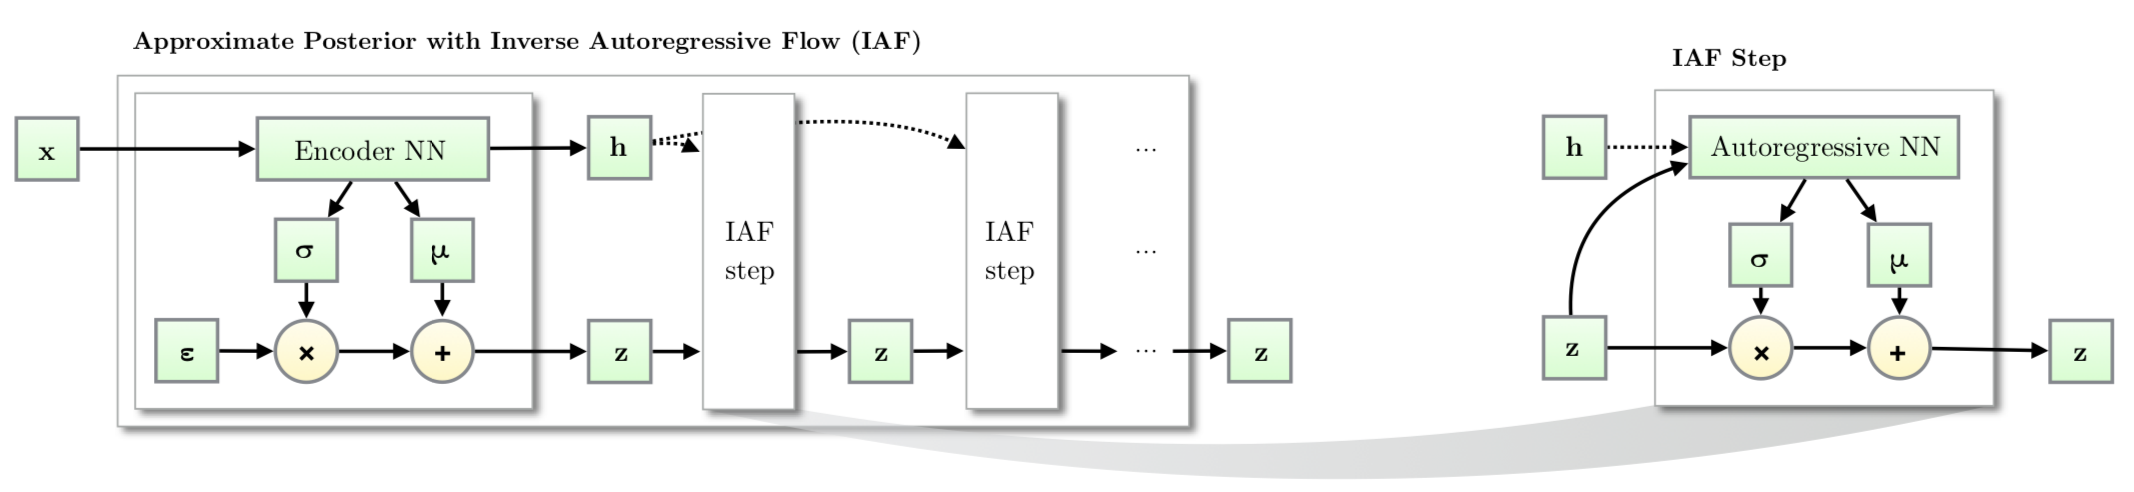
\includegraphics[width=\linewidth]{figs/iaf2.png}
	\end{figure}
	
	\myfootnotewithlink{https://arxiv.org/abs/1505.05770}{Rezende D. J., Mohamed S. Variational Inference with Normalizing Flows, 2015} 
\end{frame}
%=======
\begin{frame}{Flows-based VAE prior vs posterior}
	\begin{block}{Theorem}
		VAE with the flow-based prior $p(\bz | \blambda)$ for latent code $\bz^*$ is equivalent to VAE with flow-based posterior $q(\bz | \bx, \bphi, \blambda)$ for latent code $\bz$.
	\end{block}
	\begin{block}{Proof}
		\vspace{-0.5cm}
		\begin{align*}
			\mathcal{L}(\bphi, \btheta, \blambda) &= \mathbb{E}_{q(\bz | \bx, \bphi)} \log p(\bx | \bz, \btheta) - \underbrace{KL( q(\bz | \bx, \bphi) || p(\bz | {\color{violet}\blambda}))}_{\text{flow-based prior}} \\
			& = \mathbb{E}_{q(\bz^* | \bx, \bphi, \blambda)} \log p(\bx | f(\bz^*, \blambda), \btheta) - \underbrace{KL( q(\bz^* | \bx, \bphi, {\color{violet}\blambda}) || p(\bz^*))}_{\text{flow-based posterior}}
		\end{align*}
		(Here we use Flow KL duality theorem from Lecture 5 and LOTUS)
	\end{block}
	\begin{itemize}
		\item IAF posterior decoder path: $\bz \sim p(\bz)$, $\bx \sim p(\bx|\bz, \btheta)$.
		\item AF prior decoder path: $\bz^* \sim p(\bz^*)$, $\bz = f(\bz^*, \blambda)$, $\bx \sim p(\bx|\bz, \btheta)$. 
	\end{itemize}
	\myfootnotewithlink{https://arxiv.org/abs/1611.02731}{Chen X. et al. Variational Lossy Autoencoder, 2016}
\end{frame}
%=======
\begin{frame}{Flows-based VAE prior vs posterior}
	\vspace{-0.2cm}
	\begin{figure}
		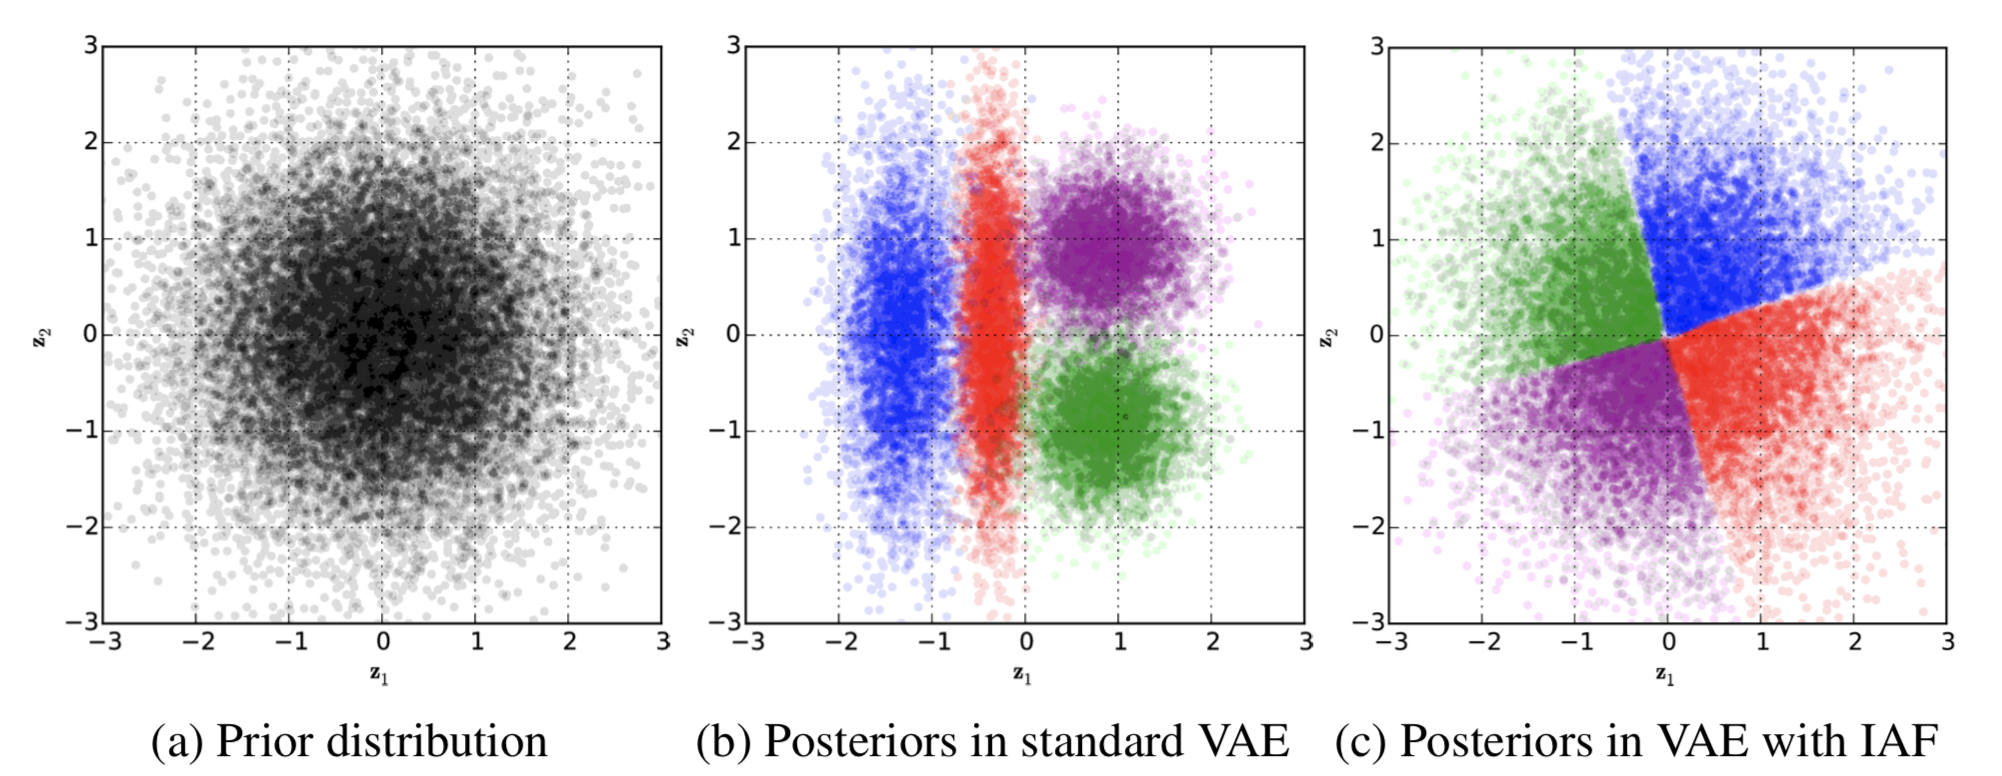
\includegraphics[width=0.9\linewidth]{figs/iaf1.png}
	\end{figure}
	\vspace{-0.3cm}
	\begin{figure}
		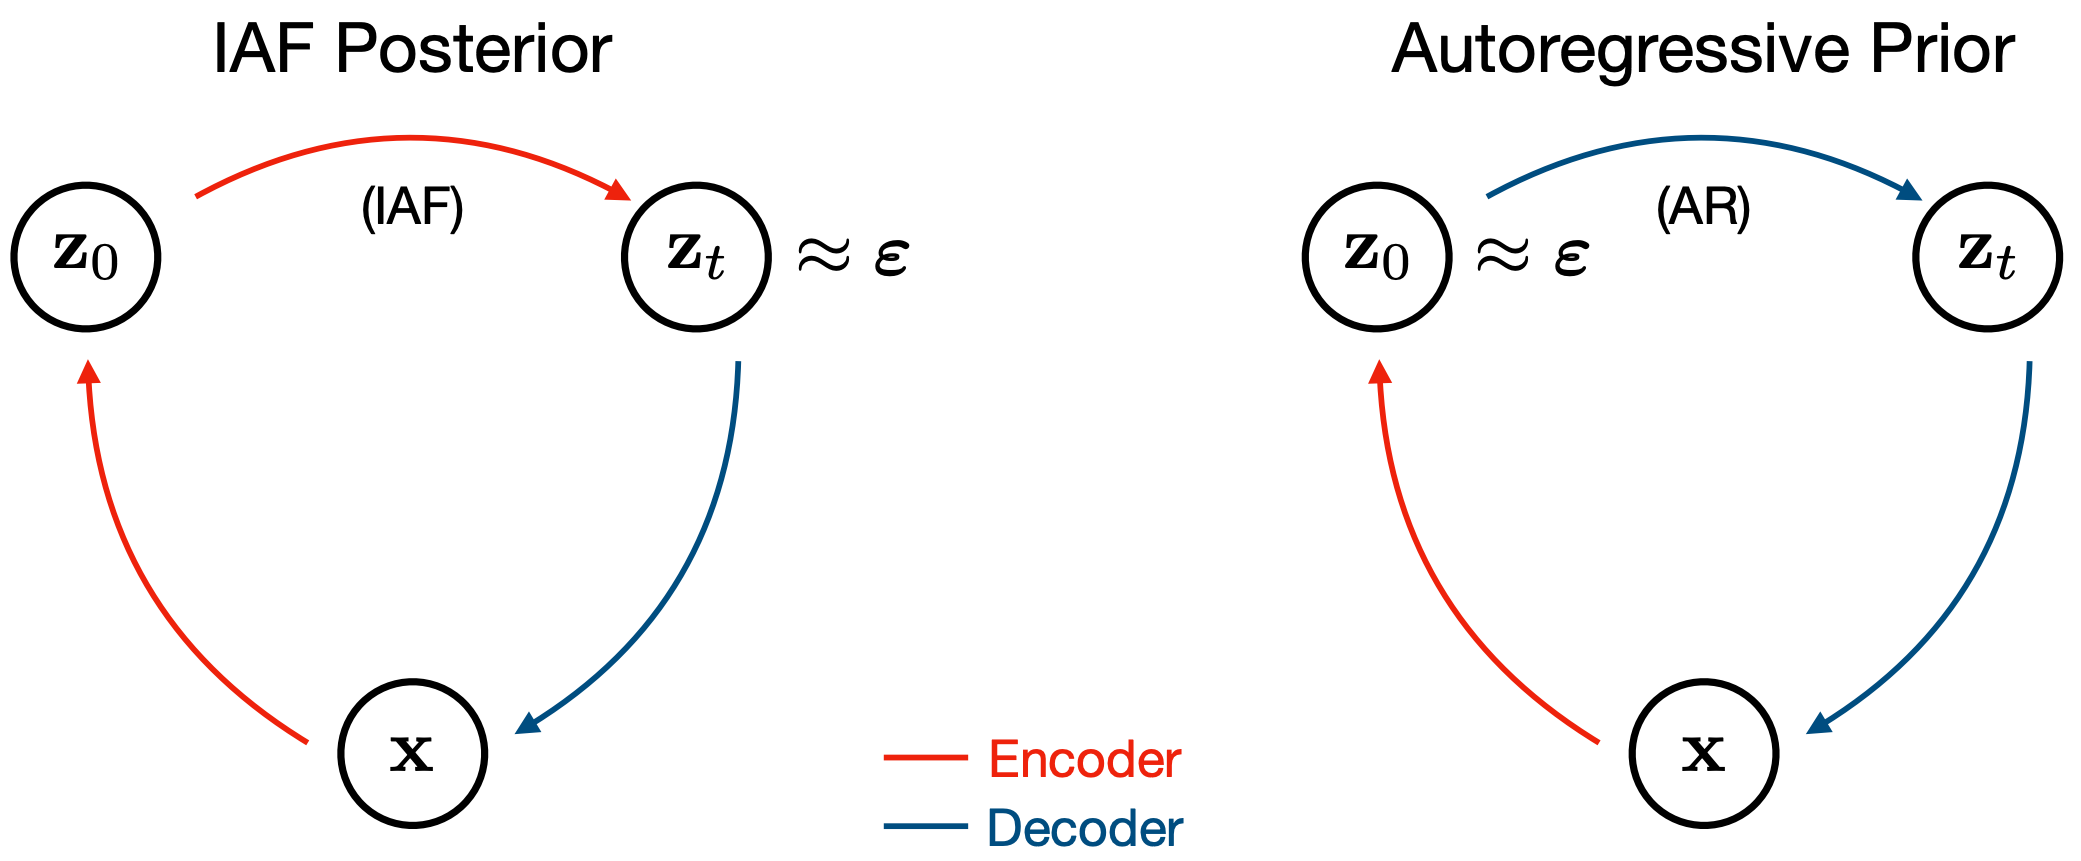
\includegraphics[width=0.65\linewidth]{figs/prior_vs_posterior}
	\end{figure}
	
	\myfootnote{\href{https://arxiv.org/abs/1606.04934}{Kingma D. P. et al. Improving Variational Inference with Inverse Autoregressive Flow, 2016} \\
		\href{https://courses.cs.washington.edu/courses/cse599i/20au/slides/L09_flow.pdf}{image credit: https://courses.cs.washington.edu/courses/cse599i/20au}}
\end{frame}
%=======
\begin{frame}{VAE limitations}
	\begin{itemize}
		\item Poor generative distribution (decoder)
		\[
		p(\bx | \bz, \btheta) = \mathcal{N}(\bx| \bmu_{\btheta}(\bz), \bsigma^2_{\btheta}(\bz)) \quad \text{or } = \text{Softmax}(\bpi_{\btheta}(\bz)).
		\]
		\item Loose lower bound
		\[
		\log p(\bx | \btheta) - \mathcal{L}(q, \btheta) = (?).
		\]
		\item Poor prior distribution
		\[
		p(\bz) = \mathcal{N}(0, \mathbf{I}).
		\]
		\item Poor variational posterior distribution (encoder)
		\[
		q(\bz | \bx, \bphi) = \mathcal{N}(\bz| \bmu_{\bphi}(\bx), \bsigma^2_{\bphi}(\bx)).
		\]
	\end{itemize}
\end{frame}
%=======
\section{Disentanglement learning}
%=======
\section{Likelihood-free learning}
%=======
\begin{frame}{Likelihood based models}
	Is likelihood a good measure of model quality?
	\begin{minipage}[t]{0.48\columnwidth}
		\begin{block}{Poor likelihood \\ Great samples}
			\vspace{-0.3cm}
			\[
				p_1(\bx) = \frac{1}{n} \sum_{i=1}^n \cN(\bx | \bx_i, \epsilon \bI)
			\]
			For small $\epsilon$ this model will generate samples with great quality, but likelihood will be very poor.
		\end{block}
	\end{minipage}%
	\begin{minipage}[t]{0.52\columnwidth}
		\begin{block}{Great likelihood \\ Poor samples}
			\vspace{-0.3cm}
			\[
				p_2(\bx) = 0.01p(\bx) + 0.99p_{\text{noise}}(\bx)
			\]
			\begin{multline*}
				\log \left[ 0.01p(\bx) + 0.99p_{\text{noise}}(\bx) \right] \geq  \\ \geq \log \left[ 0.01p(\bx) \right]  = \log p(\bx) - \log 100
			\end{multline*}
		Noisy irrelevant samples, but for high dimensions $\log p(\bx)$ becomes proportional to $m$.
		\end{block}
	\end{minipage}
	\myfootnotewithlink{https://arxiv.org/abs/1511.01844}{Theis L., Oord A., Bethge M. A note on the evaluation of generative models, 2015}
\end{frame}
%=======
\begin{frame}{Likelihood-free learning}
	\begin{itemize}
		\item Likelihood is not a perfect quality measure for generative model.
		\item Likelihood could be intractable.
	\end{itemize}
	\begin{block}{Where did we start}
	 We would like to approximate true data distribution $\pi(\bx)$.
		Instead of searching true $\pi(\bx)$ over all probability distributions, learn function approximation $p(\bx | \btheta) \approx \pi(\bx)$.
	\end{block}
	Imagine we have two sets of samples 
	\begin{itemize}
		\item $\cS_1 = \{\bx_i\}_{i=1}^{n_1} \sim \pi(\bx)$ -- real samples;
		\item $\cS_2 = \{\bx_i\}_{i=1}^{n_2} \sim p(\bx | \btheta)$ -- generated (or fake) samples.
	\end{itemize}
	\begin{block}{Two sample test}
		\vspace{-0.3cm}
		\[
			H_0: \pi(\bx) = p(\bx | \btheta), \quad H_1: \pi(\bx) \neq p(\bx | \btheta)
		\]
	\end{block}
	Define test statistic $T(\cS_1, \cS_2)$. The test statistic is likelihood free.
	If $T(\cS_1, \cS_2) < \alpha$, then accept $H_0$, else reject it.
\end{frame}
%=======
\begin{frame}{Likelihood-free learning}
	\begin{block}{Two sample test}
		\vspace{-0.5cm}
		\[
			H_0: \pi(\bx) = p(\bx | \btheta), \quad H_1: \pi(\bx) \neq p(\bx | \btheta)
		\]
		\vspace{-0.8cm}
	\end{block}
	\begin{block}{Desired behaviour}
		\begin{itemize}
			\item $p(\bx | \btheta)$ minimizes the value of test statistic~$T(\cS_1, \cS_2)$.
			\item It is hard to find an appropriate test statistic in high dimensions. $T(\cS_1, \cS_2)$ could be learnable.
		\end{itemize}
	\end{block}
	\vspace{-0.3cm}
	\begin{block}{GAN objective}
		\begin{itemize}
			\item \textbf{Generator:} generative model $\bx = G(\bz)$, which makes generated sample more realistic.
			\item \textbf{Discriminator:} a classifier $D(\bx) \in [0, 1]$, which distinguishes real samples from generated samples.
		\end{itemize}
		\[
			\min_{G} \max_D V(G, D) = \min_{G} \max_D \left[ \bbE_{\pi(\bx)} \log D(\bx) + \bbE_{p(\bz)} \log (1 - D(G(\bz))) \right]
		\]
	\end{block}
	 \myfootnotewithlink{https://arxiv.org/abs/1406.2661}{Goodfellow I. J. et al. Generative Adversarial Networks, 2014}
\end{frame}
%=======
\section{Generative adversarial networks}
%=======
\begin{frame}{Generative models zoo}
	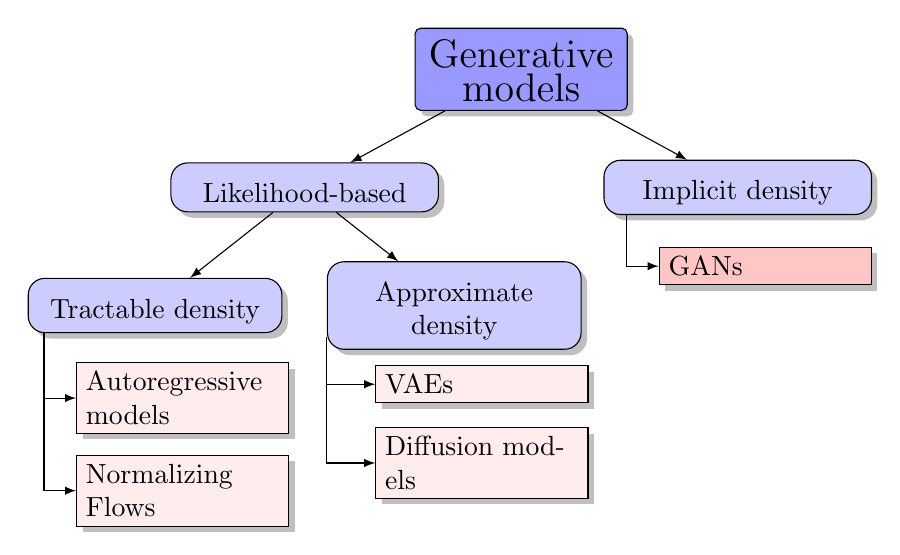
\begin{tikzpicture}[
	 	basic/.style  = {draw, text width=2cm, drop shadow, rectangle},
	 	root/.style   = {basic, rounded corners=2pt, thin, text height=1.1em, text width=7em, align=center, fill=blue!40},
	 	level 1/.style={sibling distance=55mm},
	 	level 2/.style = {basic, rounded corners=6pt, thin, align=center, fill=blue!20, text height=1.1em, text width=9em, sibling distance=38mm},
	 	level 3/.style = {basic, rounded corners=6pt, thin,align=center, fill=blue!20, text width=8.5em},
	 	level 4/.style = {basic, thin, align=left, fill=pink!30, text width=7em},
	 	level 5/.style = {basic, thin, align=left, fill=pink!90, text width=7em},
		edge from parent/.style={->,draw},
		>=latex]
		
		% root of the the initial tree, level 1
		\node[root] {\Large Generative models}
		% The first level, as children of the initial tree
		child {node[level 2] (c1) {Likelihood-based}
			child {node[level 3] (c11) {Tractable density}}
			child {node[level 3] (c12) {Approximate density}}
		}
		child {node[level 2] (c2) {Implicit density}};
		
		% The second level, relatively positioned nodes
		\begin{scope}[every node/.style={level 4}]
		\node [below of = c11, yshift=-5pt, xshift=10pt] (c111) {Autoregressive models};
		\node [below of = c111, yshift=-5pt] (c112) {Normalizing Flows};
		
		\node [below of = c12, xshift=10pt] (c121) {VAEs};
		\node [below of = c121] (c122) {Diffusion models};
		
		\end{scope}
		
		% The second level, relatively positioned nodes
		\begin{scope}[every node/.style={level 5}]
		\node [below of = c2, xshift=10pt] (c21) {GANs};
		\end{scope}
		
		
		% lines from each level 1 node to every one of its "children"
		\foreach \value in {1,2}
		\draw[->] (c11.194) |- (c11\value.west);
		
		\foreach \value in {1,2}
		\draw[->] (c12.194) |- (c12\value.west);
		
		\draw[->] (c2.194) |- (c21.west);
		
	\end{tikzpicture}
\end{frame}
%=======
\begin{frame}{Vanilla GAN optimality}
	\begin{block}{Theorem}
	The minimax game 
		\vspace{-0.1cm}
		\[
			\min_{G} \max_D V(G, D) = \min_{G} \max_D \left[ \bbE_{\pi(\bx)} \log D(\bx) + \bbE_{p(\bz)} \log (1 - D(G(\bz))) \right]
		\]
	has the global optimum $\pi(\bx) = p(\bx | \btheta)$, in this case $D^*(\bx) = 0.5$.
	\end{block}
	\begin{block}{Proof (fixed $G$)}
		\vspace{-0.5cm}
		\begin{align*}
			V(G, D) &= \bbE_{\pi(\bx)} \log D(\bx) + \bbE_{p(\bx | \btheta)} \log (1 - D(\bx)) \\
			&= \int \underbrace{\left[ \pi(\bx) \log D(\bx) + p(\bx | \btheta)\log (1 - D(\bx) \right]}_{y(D)} d \bx
		\end{align*}
		\vspace{-0.2cm}
		\[
			\frac{d y(D)}{d D} = \frac{\pi(\bx)}{D(\bx)} - \frac{p(\bx | \btheta)}{1 - D(\bx)} = 0 \quad \Rightarrow \quad D^*(\bx) = \frac{\pi(\bx)}{\pi(\bx) + p(\bx | \btheta)}
		\]
	\end{block}
	\myfootnotewithlink{https://arxiv.org/abs/1406.2661}{Goodfellow I. J. et al. Generative Adversarial Networks, 2014}
\end{frame}
%=======
\begin{frame}{Vanilla GAN optimality}
	\begin{block}{Proof continued (fixed $D = D^*$)}
		\vspace{-0.5cm}
		\begin{multline*}
			V(G, D^*) = \bbE_{\pi(\bx)} \log \frac{\pi(\bx)}{\pi(\bx) + p(\bx | \btheta)} + \bbE_{p(\bx | \btheta)} \log \frac{p(\bx | \btheta)}{\pi(\bx) + p(\bx | \btheta)} \\
		 = KL \left(\pi(\bx) || \frac{\pi(\bx) + p(\bx | \btheta)}{2}\right) + KL \left(p(\bx | \btheta) || \frac{\pi(\bx) + p(\bx | \btheta)}{2}\right) - 2\log 2 \\
		 = 2JSD(\pi(\bx) || p(\bx | \btheta)) - 2\log 2.
		\end{multline*}
	\end{block}
	\vspace{-0.3cm}
	\begin{block}{Jensen-Shannon divergence (symmetric KL divergence)}
		\vspace{-0.2cm}
		\footnotesize
		\[
			JSD(\pi(\bx) || p(\bx | \btheta)) = \frac{1}{2} \left[KL \left(\pi(\bx) || \frac{\pi(\bx) + p(\bx | \btheta)}{2}\right) + KL \left(p(\bx | \btheta) || \frac{\pi(\bx) + p(\bx | \btheta)}{2}\right) \right]
		\]
	\end{block}
	Could be used as a distance measure!
	\[
		V(G^*, D^*) = -2\log 2, \quad \pi(\bx) = p(\bx | \btheta).
	\]
	
	 \myfootnotewithlink{https://arxiv.org/abs/1406.2661}{Goodfellow I. J. et al. Generative Adversarial Networks, 2014}
\end{frame}
%=======
\begin{frame}{Vanilla GAN optimality}
	\begin{block}{Theorem}
		The minimax game 
		\vspace{-0.1cm}
		\[
			\min_{G} \max_D  V(G, D) = \min_{G} \max_D \left[ \bbE_{\pi(\bx)} \log D(\bx) + \bbE_{p(\bz)} \log (1 - D(G(\bz))) \right]
		\]
		has the global optimum $\pi(\bx) = p(\bx | \btheta)$, in this case $D^*(\bx) = 0.5$.
	\end{block}
	\vspace{-0.2cm}
	\begin{block}{Proof}
	for fixed $G$:
	\[
		D^*(\bx) = \frac{\pi(\bx)}{\pi(\bx) + p(\bx | \btheta)}
	\]
	\vspace{-0.5cm} \\
	for fixed $D = D^*$:
	\[
		\min_{G} V(G, D^*) = \min_{G} \left[ 2 JSD(\pi || p) - \log 4 \right] = -\log 4, \quad \pi(\bx) = p(\bx | \btheta).
	\]
	\vspace{-0.6cm}
	\end{block}
	If the generator could be any function and the discriminator is optimal at every step, then the generator is guaranteed to converge to the data distribution.
	 \myfootnotewithlink{https://arxiv.org/abs/1406.2661}{Goodfellow I. J. et al. Generative Adversarial Networks, 2014}
\end{frame}
%=======
\begin{frame}{Vanilla GAN}
	\begin{block}{Objective}
		\vspace{-0.4cm}
		\[
		\min_{G} \max_D V(G, D) = \min_{G} \max_D \left[ \bbE_{\pi(\bx)} \log D(\bx) + \bbE_{p(\bz)} \log (1 - D(G(\bz))) \right]
		\]
		\vspace{-0.4cm}
	\end{block}

	\begin{figure}
		\centering
		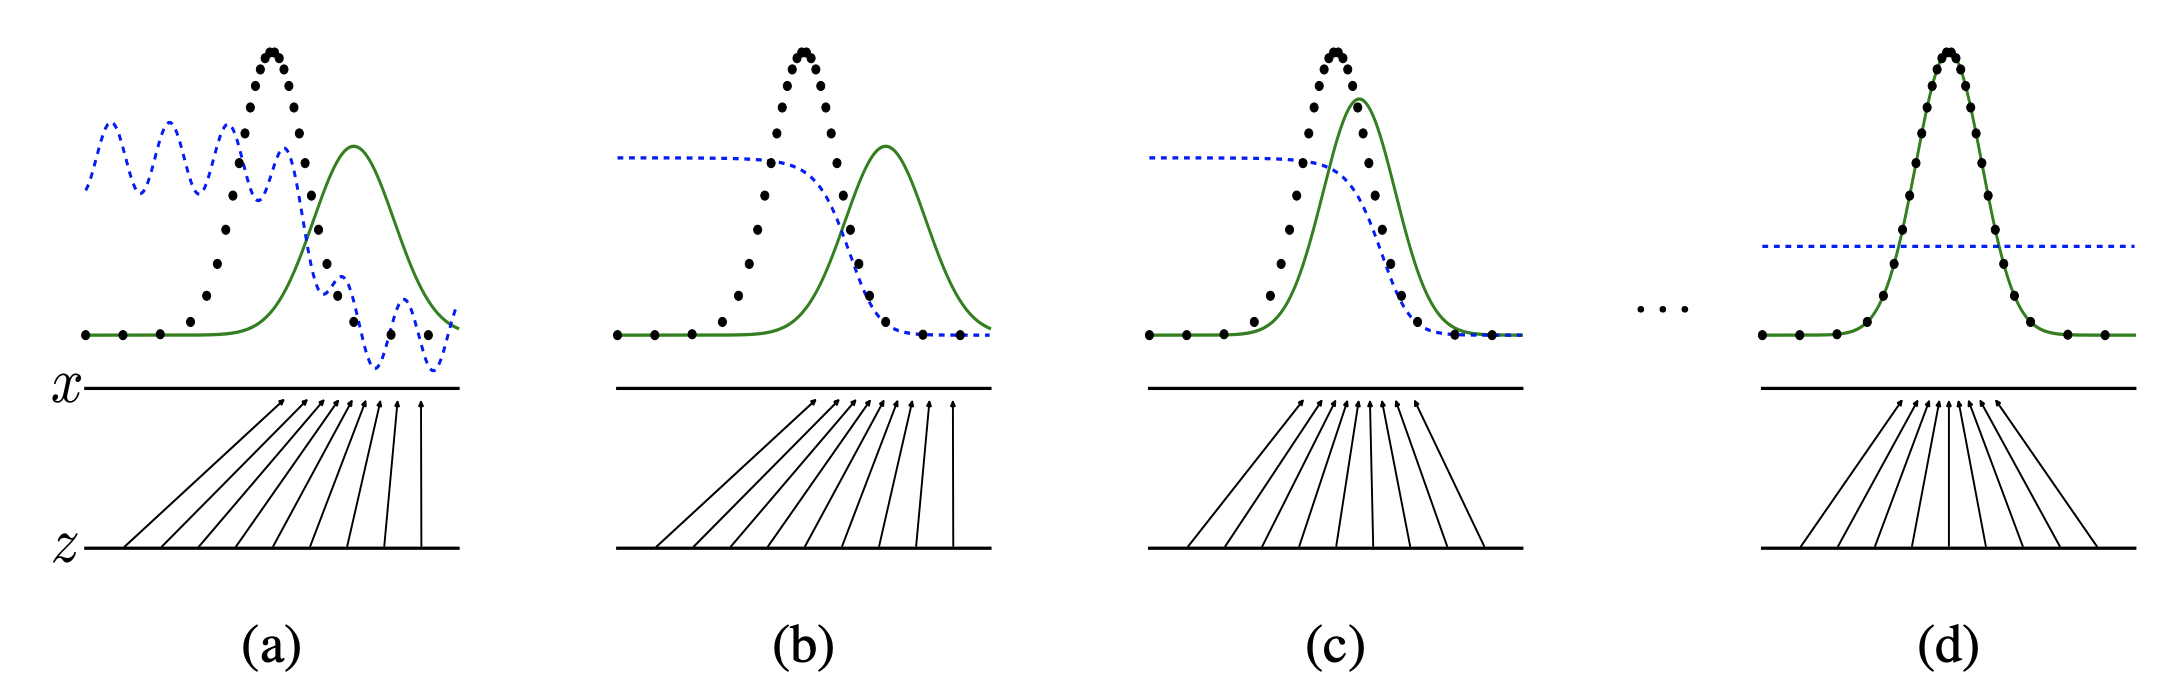
\includegraphics[width=1.0\linewidth]{figs/gan_1}
	\end{figure}
	\begin{itemize}
		\item Generator updates are made in parameter space.
		\item Discriminator is not optimal at every step.
		\item Generator and discriminator loss keeps oscillating during GAN training.
	\end{itemize}

	 \myfootnotewithlink{https://arxiv.org/abs/1406.2661}{Goodfellow I. J. et al. Generative Adversarial Networks, 2014}
\end{frame}
%=======
\begin{frame}{Summary}
	\begin{itemize}
		\item It is possible to use flows in VAE prior and posterior. This is almost the same. 
		\vfill
		\item Disentanglement learning tries to make latent components more informative.
		\vfill
		\item $\beta$-VAE makes the latent components more independent, but the reconstructions get poorer. DIP-VAE does not make the reconstructions worse using ELBO surgery theorem.
		\vfill
		\item Majority of disentanglement learning models use heuristic objective or regularizers to achieve the goal, but the task itself could not be solved without good inductive bias.
		\vfill
		\item Likelihood is not a perfect criteria to measure quality of generative model.
		\vfill		
		\item Adversarial learning suggests to solve minimax problem to match the distributions.
		\vfill
		\item Vanilla GAN tries to optimize Jensen-Shannon divergence (in theory).
	\end{itemize}
\end{frame}
\end{document} 